\documentclass{school-22.211-notes}
\date{April 11, 2012}

\begin{document}
\maketitle

\lecture{Fuel Depletion} \label{fuel-depletion}
For fuel assembly depletion, the reactivity of fuel changes dramatically with burnup. 

\topic{Actinide Chain Construction}
Normally we would model around 400 actinides; for this class, we only discuss 22 of them, which occupies the high-end of actinides (with large N, large Z). 

What happens during actinide chain construction? 
\begin{enumerate}
\item Fission product absorptions reduce reactivitiy of the fuel significantly, often 10-20\%;
\item \ce{^{235}U} depletion significantly ...

\item Fission cross section: isotopes have threshold energies, producing step-shape near higher energies (around 10 MeV)\footnote{Both even and odd isotopes have threshold energies, but odd isotopes have higher resonance fission cross section, hence even isotopes' threshold energy behavior is more pronoud.}. Remember Pu is very fissile material. Am242 is a funny one -- although it's an even isotope, its fission cross section is large. 

\item Simple actinide nuclide transmutation model. In Figure, the red arrors designate the actinide chains we model (chains end at isotopes that decay quickly compared with the phenomena we are trying to model); blue arrors designate beta decay. 

\item The higher you go up the chain (e.g., into the MA region), the worse the absorption would be. 

\item Branching ratio is a function of energy. Example: \ce{^{241}Am} can produce \ce{^{242}Am} with a half-life of 16 hrs, and the meta-stable \ce{^{242m}Am} with a half-life of 141 years. \ce{^{242}Am}'s thermal branching ratio is about 10\% that of \ce{^{242m}Am}. 
\end{enumerate}


\clearpage
\topic{Actinide Chain Solutions}
Recall our nuclide balance equation. For this model, we do not have the `direct production by fission' term anymore.  No fission yield term. 

Compare fission product matrix form vs. actinides matrix formin Fig.~\ref{fp-an-matrix-form} : 
\begin{figure}[ht]
  \centering
  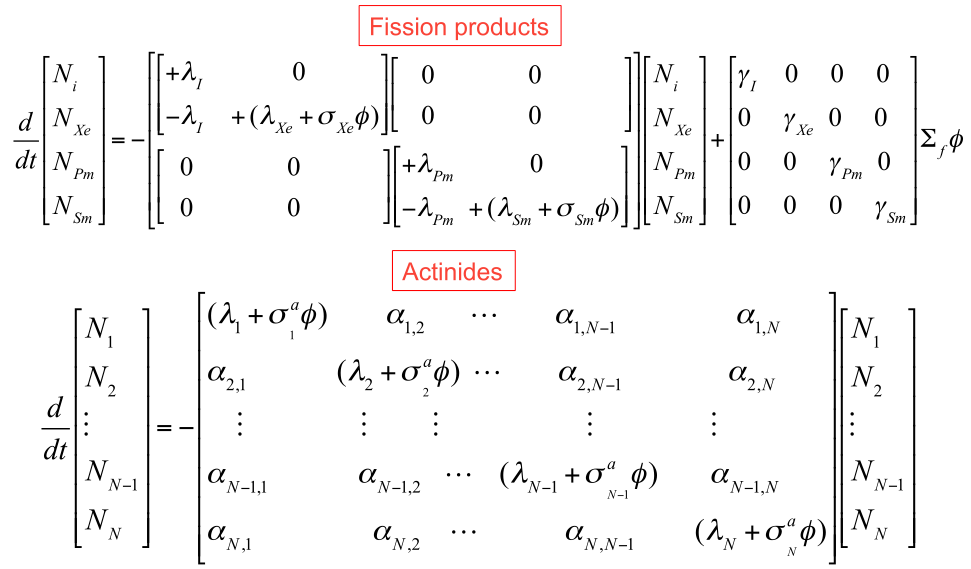
\includegraphics[width=5in]{images/dfs/fp-an-matrix-form.png}
  \caption{Nuclide Depletion Equations vs. Actinide in Matrix Form} \label{fp-an-matrix-form}
\end{figure}
\begin{itemize}
\item Actinides matrix form has no fission yield term;
\item Fission product matrix is decoupled; actinide matrix is not; 
\end{itemize}


More specifically, we focus on the actinides matrix, and notice: blue circles are decay coupling term; a n2n reaction with isotope 2 produces isotopes 1. 

\begin{figure}[ht]
  \centering
  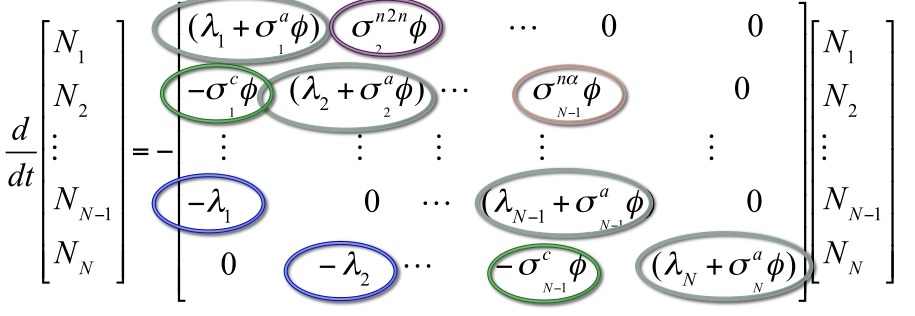
\includegraphics[width=5in]{images/dfs/nuclide-depletion-matrix-form.png}
  \caption{Nuclide Depletion Equations vs. Actinide in Matrix Form} \label{nuclide-depletion-matrix} 
    \end{figure}


There are 4 blocks for the 4 species as in Fig.~\ref{actinide-block}. 
\begin{figure}[ht]
  \centering
  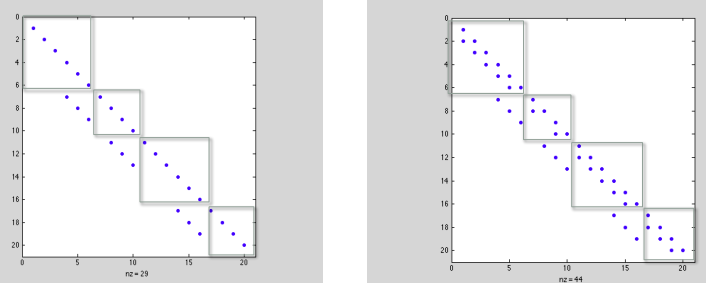
\includegraphics[width=5in]{images/dfs/actinide-block.png}
  \caption{Matrix Shape for Actinide Depletion Equations} \label{actinide-block} 
    \end{figure}
\begin{itemize}
\item The decay terms sit outside of the blocks; they couple the blocks.
\item  The capture terms are one line off the diagonal term (NP238 decays so quickly that its capture cross section is zero and is not shown throug the spy function in matlab); 
\item We don't have above the diagonal term because we ignore the $n2n$ reaction and the $n \alpha$ reaction. The reason we ignore them is that having a sub-diagonal matrix we can invert analytically; whereas having a full matrix is a lot harder to invert. Another simplification we made is to ignore all meta-stable states and only have the ground states, hence ignoring branching. 
\end{itemize}

\textbf{Understanding the solutions we obtained}:
\begin{enumerate}
\item U238 barely changes; there are a lot of it, and it probably decreases by 1\%; often time the nuclear concentration is plotted with respect to initial heavy metal inventory, that is, U238 concentration. 
\item U234, U235 does not have production, hence it decreases. 
\item U236 is produced as we burnup U235; U236 has almost no destruction rates;
\item U237 is produced as we burnup 
\item U239 is a constant because its capture from U238 is constant, and U239 decays so quickly (23 mins) that it's at equilibrium the whole time. 
\item (remember) Np has a half-life of 2 and 2.5 days; Np's cancels out Am etc, and they have the same half-life, so people use to ignore them. 
\item Production with Pu; 
\item Am244: takes a certain burnup to come up. Even though Am is a small concentration, we still care about them. 
\end{enumerate}

About 40-50\% of power would be produced from Pu instead of U by the time we shut down the reactor. 





\clearpage
\topic{Burnup Units}
\begin{enumerate}
\item FIFA = fission per initial fissile atoms;
\item FIMA = fission per initial (heavy) metal atoms;
\item Atom percent (A\%) = FIMA * 100;
\item Burnup: GWd/T = MWd/kg = thermal power per weight of heavy metal. 
  \begin{itemize}
    \item Advantages: we know the reactor power and 
    \item Disadvantages: `energy released' is not a very clean term; we don't really care about neutrino energy, gamma energy released from capture of neutrons; energy deposited in fuel assembly B from fissions in assembly A. In LWR, it is a good approximation to assume that energy is depositied where the fission is; in MITR it is a bad approximation, fission product energy (deposite locally), gamma heat energy (not necessarily deposited locally), etc. 
  \end{itemize}
\item EFPHs = Effective Full Power Hours; EFPD = Effective Full Power Days. 
\end{enumerate}

\clearpage
\topic{Numerous Subtle Effects}
\begin{enumerate}
 \item We didn't really cover the Thorium/U233 Chain in Kord's class. 
   \begin{itemize}
   \item The chain for Th is very complicated; there are n2n reactions at all different levels; there are multiple ways to get U232; 
   \item some of these isotopes have very rapid alpha decays; 
   \item Pa233 has 27 day half-life; 
   \item U232 has 70 year half-life; U232's daughter product Ta208 has 2.6 MeV gamma (which is the hardest gamma known). 
   \end{itemize}
   Coverage of Th/U233 comparison from Ben's class (11/29). [FIXME]


\item Burnable Poisons History Effect: hardern the spectrum, because it pushes some water away, BP history effect: you place BP in it at the beginning of the reactor, we take it out later hence to achieve flat power through time. The BP effect is about 250 pcm. 

\item Fuel Temperature Depletion History Effects: 
Initially, the instantenous temperature effect is almost independent of depletion; as the burnup increases, something happens. The moral of the story is, we not only need to know the burnup but also the temperature. 

\item Gadolinium burnable absorber: 
  \begin{itemize}
  \item Gadolinium has a huge thermal absorption cross section. It's almost as high as Zn, but we cannot use Zinon because it would ecay; 
  \item What we do with Gadolinium is to replace part of the fuel with Gad and reactivity would be flatter with respect to time. 
  \item Hold-down is the difference between the reactivity at the beginning of life-cycle. 
  \item Gad resdual: there is a little bit loss of reactivity due to Gad. Gad depletes from outside to inside. 
  \end{itemize}


\item Where do reaction rates come from? 
  \begin{itemize}
  \item ORIGEN uses point depletion, 
  \item Fuel pin radial shape: the outter region almost have 2 times the flux compared with the inner ones. 
  \end{itemize}

\item Benchmark: 
  \begin{itemize}
  \item data set is the single most important things in determine the accuracy of your codes.
  \item U235 has a pretty large error, but we don't care because there is so little of it;
  \item Accuracy tends to decrease the further up the decay chains. 
  \item Measurements also have an intrinsic uncertainty; do not rely on single measurement campaigns; systematic errors in measurements are common. 
  \item In performing `actinide burner' analysis, when we place the actinide at the end of one analysis into another one, the error builds up. 
  \end{itemize}
\end{enumerate} 



\clearpage
\topic{Spent Fuel and Recycling}
This lecture was given by Prof. Forget on 11/29/12. 
\begin{enumerate}

\item Pu enrichment is higher than U enrichment for two reasons: a) only 60\% Pu is fissile \ce{^{239}Pu}, the rest of them are parisitic; b) Pu has a higher absorption rates. 

\item The majority of the spent fuel is U238 which is not real waste; the U and Pu in the spent fuel is sent back to the core. The real waste is limited to MA and is vitrified in a borosilicate glass form. 

\item Multi-recycling: we cannot recycle too many times. Reason: after 1st cycle the fissile content is 64.8\%, after 2nd cycle fissile is only 51.1\% and requires a higher Pu enrichment; and if Pu enrichment is pass xxx, then the void coefficient would become positive. 

\item DUPIC cycle (used in CANDU): it is an entirely mechanical process during which we grind up everything, the gas comes out, and re-construct the grinds into fuel which contains about 0.8\% U235 and 0.8\% Pu239, which is about twice the excess reactivity of natural uranium and is more than enough for a CANDU.

\item Fast reactor transmutation: at high energy, all MA are fissible (also high absorption cross section which is why we don't expect to get energy from MA), so we can transmutate MA.  


\item Th cycle advantages: 
\begin{enumerate}
\item Abundancy is 4x that of U. 
\item Less waste:  we start further bottom left from the chain, and Th cycle would generate less MA waste. 

\end{enumerate}
Companies that considers Th cycle: Thorium Power Inc which is a subsidiary of Lightbridge Corp. 
\end{enumerate}

\clearpage
\topic{Relate Neutronics and TH}
This lecture was given by Prof. Forget on 12/04/12. 
\begin{enumerate}
\item FP deposit energy locally, and fuel expands due to temperature changes. Because the temperature increase on the inside is larger than the outside, pellets are fabricated with a slightly shorter height on the inside as in Fig.~\ref{fuel_pellets}
\begin{figure}[ht]
  \centering
  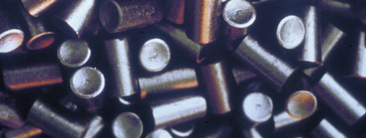
\includegraphics[width=4in]{images/dfs/fuel_pellets.png}
  \caption{Fuel Pellets Shapes} \label{fuel_pellets}
\end{figure}


\item \ce{UO_2} is used in LWRs regardless of its low heat transfer property because it does not interact with water violently. \ce{UO_2} has a relatively low thermal expand, so the gap between the fuel and the clad can be relatively small. 

\item Fast reactors use metallic fuel because a) better heat transfer, b) coolant is not water so no worry for chemical reaction, c) metallic fuel thermal expansion is large, which replaces Doppler effect(recall Doppler is due to U238 -- ). Also because metallic fuel expands more, we build fuel pellets with more porosity to limit the amount of volume expansion. 

\item Grid straps: egg crates to place pins in them. Pin starts vibrating and may cause fuel failure. 

\item To flattern power peaking: 
  \begin{enumerate}
  \item Core loading. 
  \item Poisons: WABA, IFBA \ce{Zr B_2}, Gd and other Lanthanum. 
  \item Control rod sequence. 
  \item Reflector. 
  \item Core enrichment. 
  \item Flow orificing: change flow pattern at different assemblies. It is not done in LWRs that often, more common in SFRs to control temperature and flux spectrum. 
  \end{enumerate}

\item Thermal transients in fuel: 
  \eqn{ M_F C_{p,f} \frac{\dT_f}{\dt} = P(t) - \frac{1}{R_f} (T_f(t) - T_c(t)) }
  where $R_f$ captures all the thermal resistance. Assume steady state, then 
  \eqn{ P(t) =  \frac{1}{R_f} (T_f(t) - T_c(t)) }
  If we assume a fast transient with no cooling ($R_f \to \infty$), then we get adiabatic heat rate:
  \eqn{ M_f C_{p,f} \frac{\dT_f}{\dt} = P(t) }


\item Thermal transients in coolant: 
  \eqn{ M_C C_{p_C} \frac{\dT_c}{\dt} = \frac{1}{R_f} (T_f(t) - T_c(t)) - 2 \dot{m}_c C_{p_c} (T_c(t) - T_i) }
  where $\dot{m}$= mass flow of coolant, and the factor of $2$ is there because the $T_c(t)$ in the equation is assumed to be the average. 
  \begin{itemize}
    \item Steady state: $\displaystyle 2 \dot{m} C_{P_c} (T_c - T_i) = \frac{1}{R_f} (T_f - T_c) = P$. That is, reactor power is determined from flow and temperature measurements. 
  \end{itemize}


\item We can relate the above two equations with the PKE using $P(t)$. That is, how do we relate temperature change to reactivity change. 
  \begin{enumerate}
    \item Set-up: consider $\displaystyle \rho = \frac{k-1}{k}, \drho = \frac{\dk}{k^2}$. If we assume $k \approx 1$, then $\displaystyle \drho =  \frac{\dk}{k} = \derivative(\ln k)$. There is benefit in writing $k$ in log form as now we can separate multiplication into additions. 

  \item Consider $\keff = \kinf P_{NL}$, where $P_{NL} = \frac{1}{L^2 B_g^2}$, we can write, 
    \eqn{ \derivative (\ln k) = \derivative(\ln \kinf) + \derivative(\ln P_{NL}) = \frac{\dk_{\infty}}{\kinf} + \frac{\dP_{NL}}{P_{NL}} }
    We can do: 
    \eqn{\frac{\dP_{NL}}{P_{NL}} = - \frac{L^2 B_g^2}{1 +L^2 B_g^2} \left( \frac{\derivative L^2}{L^2} + \frac{\derivative B_g^2}{B_g^2} \right) }

  \item Recall 
    \eqn{ \kinf = 
\overbrace{\left( 1 + \frac{\nu \Sigma_{f1}}{\nu \Sigma_{f2}}  \frac{\Sigma_{a2} + D_2 B_g^2}{\Sigma_{12}} \right)}^{\epsilon} 
\overbrace{\frac{\Sigma_{s12}}{\Sigma_{R1}}  }^{\rho} 
\overbrace{\frac{\nu \Sigma_{f2}^F}{\Sigma_{a2}^F} }^{\eta} 
\overbrace{\frac{\Sigma_{a2}^F}{\Sigma_{a2}}}^{f} }

    \item If we characterize the temperature effect as $\kinf = f(T_m, T_f, T_m)$. For PWR $T_m = T_c$, 
      \eqn{ \drho = \frac{\dk_{\infty}}{\kinf} = \frac{1}{\kinf} \frac{\derivative \kinf}{\dT_f} + \frac{1}{\kinf} \frac{\derivative \kinf}{\dT_c} }
      If we define reactor coefficient, 
      \eqn{ \alpha_x = \frac{1}{\kinf} \frac{\dk_{\infty}}{\dT_x} = \frac{1}{\epsilon} \frac{\derivative \epsilon}{\dT_x} + \frac{1}{\rho} \frac{\drho}{\dT_x} +  \frac{1}{f} \frac{\derivative f}{\dT_x} +  \frac{1}{\eta} \frac{\derivative \eta}{\dT_x} }


    \item Fuel temperature feedback: Doppler (Doppler broadening of resonances capture of \ce{^{238}U}, 
      \begin{itemize}
      \item Impact $\rho$ (resonance escape probability): 
      \eqn{ \rho &= \frac{\Sigma_{s12}}{\Sigma_{R1}} & T_f &\up, \Sigma_{R1} \up, \rho \down} 
    \item Impact $\epsilon$ is negliable above resonance region. 
    \item Impact $\eta = \frac{\nu \Sigma_f^F}{\Sigma_{a2}^F}$ is very small because fission and absorption cross section scales with temperature approximately the same. 
    \item Impact on $f= \frac{\Sigma_{a2}^F}{\Sigma_{a2}}$ is very small because absorption cross section scales with temperature approximately the same in fuel and outside the fuel.
    \item PWR has a $\alpha_f = -0.01$ to $-0.03$ mk/degreeC. SFR is about the same. 
      \end{itemize}
      
    \item Moderator temperature. Consider $T_m = T_c$ for PWR, 
      \eqn{ \alpha_m = \frac{1}{\kinf} \frac{\dk_m}{\dT_m}  \approx \frac{1}{\kinf} \frac{\dk_{\infty}}{\dN_m} \frac{\dN_m}{\dT_m} }
      There is no resonance effect; temperature effect is felt through density change. 
      \begin{itemize}
      \item We define expansion coefficient (volume changes at constant pressure) 
        \eqn{ \beta_m &= - \frac{1}{N_m} \frac{\dN_m}{dT_m} & \alpha_m = - \beta_m N_m \frac{1}{\kinf} \frac{\dk_{\infty}}{\dN_m}  }

      \item The expansion coefficient of sodium and salt is very large; it will change density, cross section, and push some coolant outside thus changing the moderator-to-fuel ratio. 

      \item For our case, two terms depend on the fuel and do not change much: $\epsilon, \eta$. Most of the effect is felt by resonance escape probability $p$ and thermalization factor $f$. 

      \item In $p$, $\Sigma_{s12} = N_m \sigma_{H, s12}$ changes as water density changes. The cross sections are considered flat. 

      \item In $f$, $\displaystyle f = \frac{\Sigma_{a2,F}}{\Sigma_{a2}} = \frac{\Sigma_{a2, F}}{\Sigma_{a2,F} + \Sigma_{a2, M} + \Sigma_{a2, CC} + \Sigma_{a_2, SB}} $, where $\Sigma_{a2,M}$ does not change much because moderator's absorption cross section is relative small compare with control rods and soluble boron's absorption cross sections. As $T_c \up$, water density decreases, $N_{SB} \down, f \up$. The effect of control rod is more subtle -- as $T_c \up$, water density decreases, water moderates less, spectrum hardens, then the dominating cross section becomes smaller (recall 1/v behavior in absorption cross section in thermal energy range). \textcolor{blue}{This is a good way to consider spetral effect: think about how the flux peak shifts, and think what the cross section is like at that peak.}
        
      \item Summary: as $T_c \up, p \down, f \up$. 
      \end{itemize}

  \end{enumerate}
\end{enumerate}



\end{document}
